%===========================================================================
%  Agentic Restaurant Customer Service System — NLP Course Report
%  CSE389 (UG2023) — Natural Language Processing
%===========================================================================
\documentclass[12pt,a4paper]{report}

% ── Packages ───────────────────────────────────────────────────────────────
\usepackage[T1]{fontenc}
\usepackage[utf8]{inputenc}
\usepackage{lmodern}
\usepackage[margin=2.5cm]{geometry}
\usepackage{graphicx}
\usepackage{float}
\usepackage{booktabs}
\usepackage{tabularx}
\usepackage{array}
\usepackage{multirow}
\usepackage{xcolor}
\usepackage{hyperref}
\usepackage{tikz}
\usetikzlibrary{positioning}
\usepackage{enumitem}
\usepackage{fancyhdr}
\usepackage{titlesec}
\usepackage{caption}
\usepackage{subcaption}
\usepackage{listings}
\usepackage{upquote}
\usepackage{amsmath}
\usepackage{setspace}
\usepackage{parskip}
\usepackage{microtype}
\usepackage{mdframed}
\usepackage{pifont}
\newcommand{\cmark}{\ding{51}}
\newcommand{\xmark}{\ding{55}}

% ── Colour palette ─────────────────────────────────────────────────────────
\definecolor{primary}{RGB}{31, 73, 125}
\definecolor{accent}{RGB}{192, 80, 77}
\definecolor{lightgray}{RGB}{245, 245, 245}
\definecolor{codegray}{RGB}{100, 100, 100}
\definecolor{nodecolor}{RGB}{70, 130, 180}
\definecolor{edgecolor}{RGB}{80, 80, 80}

% ── Hyperref setup ─────────────────────────────────────────────────────────
\hypersetup{
    colorlinks=true,
    linkcolor=primary,
    urlcolor=accent,
    citecolor=primary,
    pdftitle={Agentic Restaurant Customer Service System},
    pdfauthor={Mohamed Tarek Elsayed; Renad Sameh Ibrahim},
}

% ── Header / footer ────────────────────────────────────────────────────────
\pagestyle{fancy}
\fancyhf{}
\fancyhead[L]{\small\textcolor{primary}{\textbf{CSE389 — Natural Language Processing}}}
\fancyhead[R]{\small\textcolor{primary}{Agentic Restaurant CS System}}
\fancyfoot[C]{\thepage}
\renewcommand{\headrulewidth}{0.4pt}

% ── Section title styling ──────────────────────────────────────────────────
\titleformat{\chapter}[display]
  {\normalfont\Large\bfseries\color{primary}}
  {\chaptertitlename\ \thechapter}{12pt}{\Huge}
\titleformat{\section}
  {\normalfont\large\bfseries\color{primary}}
  {\thesection}{1em}{}
\titleformat{\subsection}
  {\normalfont\normalsize\bfseries\color{primary!80}}
  {\thesubsection}{1em}{}

% ── Code listing style ─────────────────────────────────────────────────────
\lstset{
  backgroundcolor=\color{lightgray},
  basicstyle=\ttfamily\small,
  keywordstyle=\color{primary}\bfseries,
  commentstyle=\color{codegray}\itshape,
  stringstyle=\color{accent},
  breaklines=true,
  frame=single,
  rulecolor=\color{primary!30},
  numbers=left,
  numberstyle=\tiny\color{codegray},
  captionpos=b,
}

% ── Utility box ────────────────────────────────────────────────────────────
\newmdenv[
  backgroundcolor=lightgray,
  linecolor=primary,
  linewidth=1pt,
  roundcorner=4pt,
  innerleftmargin=10pt,
  innerrightmargin=10pt,
  innertopmargin=8pt,
  innerbottommargin=8pt,
]{infobox}

% ── Graphics path ──────────────────────────────────────────────────────────
\graphicspath{{../agent_graphs/}{../metrics_visuals/}}

%===========================================================================
\begin{document}
%===========================================================================

% ── Title page ─────────────────────────────────────────────────────────────
\begin{titlepage}
\centering
\vspace*{1cm}

{\Large \textbf{\textcolor{primary}{Ain Shams University}}}\\[0.2cm]
{\large \textcolor{primary}{Faculty of Computer and Artificial Intelligence Engineering}}\\[1.2cm]

\rule{\linewidth}{1.5pt}\\[0.4cm]
{\Huge \textbf{\textcolor{primary}{Agentic Restaurant Customer\\[0.2cm] Service System}}}\\[0.3cm]
\rule{\linewidth}{1.5pt}\\[1cm]

{\Large \textit{A Multi-Agent Natural Language Processing System\\
Built with LangGraph, LangChain, and GPT-4o-mini}}\\[1.5cm]

\begin{tabular}{rl}
\textbf{Course:}    & CSE389 (UG2023) — Natural Language Processing \\[0.4cm]
\textbf{Students:}  & Mohamed Tarek Elsayed \quad \texttt{ID: 2300535}\\[0.15cm]
                    & Renad Sameh Ibrahim \quad \texttt{ID: 23p0292}\\[0.15cm]
                    & Salma Tamer Fathi \quad \texttt{ID: 23p0023}\\[0.4cm]
\textbf{Supervisor:}& Prof.\ Alaa Hmady \\[0.15cm]
\textbf{TA:}        & Nada Amr \\[0.4cm]
\textbf{Date:}      & May 2026 \\
\end{tabular}

\vfill

\begin{infobox}
\centering
\textbf{Abstract}\\[0.3cm]
\begin{flushleft}
This report presents the design, implementation, and evaluation of a multi-agent customer
service chatbot for a restaurant. The system routes every customer message through an
intent-classification orchestrator to one of four specialised sub-agents — Menu, Order,
FAQ, and Support — each modelled as a directed acyclic graph of LLM-powered and
deterministic nodes using LangGraph. A FastAPI backend, a SQLAlchemy database layer,
and a React front-end complete the production stack. The entire pipeline is evaluated
using an LLM-as-a-Judge framework that scores responses on relevance, correctness,
and helpfulness across 50 representative test cases.
\end{flushleft}
\end{infobox}

\end{titlepage}

% ── Table of contents ──────────────────────────────────────────────────────
\tableofcontents
\listoffigures
\listoftables
\newpage

%===========================================================================
\chapter{Introduction}
%===========================================================================

\section{Motivation}

The restaurant industry increasingly relies on digital channels to handle customer
inquiries, process orders, and resolve complaints at scale. Traditional rule-based
chatbots struggle with the open-ended, ambiguous nature of natural language.
This project applies modern large language model (LLM) techniques to build an
\textit{agentic} customer service assistant that can reason, plan, and act — not
merely pattern-match.

\section{Problem Statement}

A single monolithic LLM prompt cannot handle the full breadth of restaurant customer
interactions efficiently. Different types of requests (browsing the menu, placing an
order, asking about opening hours, filing a complaint) require different workflows,
tools, and database operations. The challenge is to correctly identify the user's
intent and delegate it to a sub-system optimised for that task — all while maintaining
conversational context across multiple turns.

\section{Objectives}

\begin{itemize}[leftmargin=1.5cm]
    \item Design a modular, multi-agent architecture where each agent is responsible
          for exactly one domain of customer interaction.
    \item Use LangGraph StateGraph to make agent logic explicit, inspectable, and
          testable as directed graphs of nodes and edges.
    \item Ground every agent in real database state (menu items, orders, FAQs, tickets)
          via SQLAlchemy repositories.
    \item Expose the system through a RESTful FastAPI backend consumed by a React
          single-page application.
    \item Evaluate quality objectively using an LLM-as-a-Judge scoring framework.
\end{itemize}

\section{Report Structure}

Chapter~\ref{ch:arch} describes the overall system architecture.
Chapter~\ref{ch:tech} surveys the technology stack.
Chapters~\ref{ch:orchestrator} through~\ref{ch:support} detail each agent individually.
Chapter~\ref{ch:api} covers the FastAPI backend and session management.
Chapter~\ref{ch:eval} presents the evaluation methodology and results.
Chapter~\ref{ch:conclusion} concludes with lessons learned and future directions.

%===========================================================================
\chapter{System Architecture}\label{ch:arch}
%===========================================================================

\section{High-Level Design}

The system follows a \textbf{hierarchical multi-agent} pattern:

\begin{center}
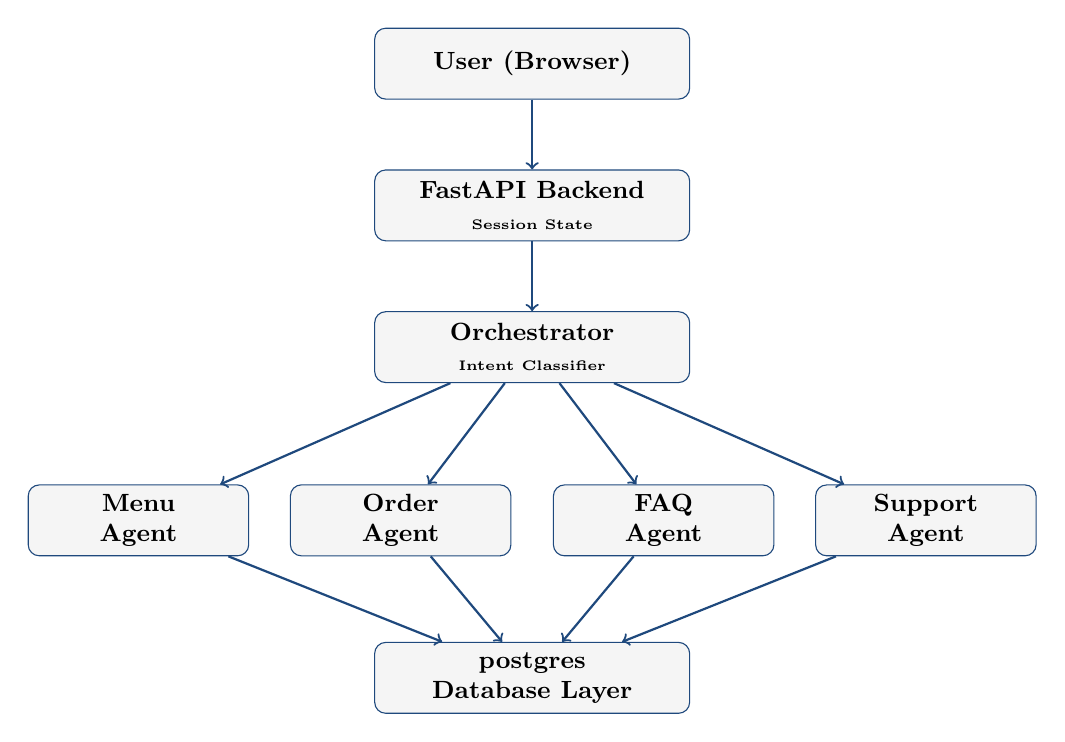
\begin{tikzpicture}[
    box/.style={draw=primary, fill=lightgray, rounded corners=4pt,
                minimum width=2.8cm, minimum height=0.9cm, align=center,
                font=\small\bfseries},
    arr/.style={->, thick, color=primary},
]
\node[box, minimum width=4cm] (user)  at (0,0)    {User (Browser)};
\node[box, minimum width=4cm] (api)   at (0,-1.8) {FastAPI Backend\\{\tiny Session State}};
\node[box, minimum width=4cm] (orch)  at (0,-3.6) {Orchestrator\\{\tiny Intent Classifier}};
\node[box] (menu)    at (-5,-5.8)  {Menu\\Agent};
\node[box] (order)   at (-1.67,-5.8) {Order\\Agent};
\node[box] (faq)     at (1.67,-5.8)  {FAQ\\Agent};
\node[box] (support) at (5,-5.8)   {Support\\Agent};
\node[box, minimum width=4cm] (db) at (0,-7.8) {postgres\\Database Layer};

\draw[arr] (user)  -- (api);
\draw[arr] (api)   -- (orch);
\draw[arr] (orch)  -- (menu);
\draw[arr] (orch)  -- (order);
\draw[arr] (orch)  -- (faq);
\draw[arr] (orch)  -- (support);
\draw[arr] (menu)    -- (db);
\draw[arr] (order)   -- (db);
\draw[arr] (faq)     -- (db);
\draw[arr] (support) -- (db);
\end{tikzpicture}
\end{center}

\section{Shared State}

All agents communicate through a single \textbf{TypedDict} called \texttt{MainState}.
LangGraph uses this as the canonical state object that is threaded through every node
invocation. Key fields include:

\begin{table}[H]
\centering
\caption{Key \texttt{MainState} Fields}
\begin{tabularx}{\textwidth}{lX}
\toprule
\textbf{Field} & \textbf{Purpose} \\
\midrule
\texttt{user\_message}              & Raw text from the customer \\
\texttt{intent}                     & Classified intent (\textit{menu / order / faq / support / off\_topic / unclear}) \\
\texttt{response}                   & Final text response returned to the user \\
\texttt{messages}                   & Full conversation history (LangChain message objects) \\
\texttt{customer\_id}               & Authenticated customer primary key \\
\texttt{extracted\_order}           & Structured order payload (items, type, address) \\
\texttt{extracted\_complaint}       & Structured complaint payload \\
\texttt{order\_awaiting\_confirmation} & Flag: pending user confirmation before placing \\
\texttt{modification\_target\_id}   & Order ID being modified across turns \\
\texttt{needs\_human}               & Flag: complaint requires human escalation \\
\texttt{faq}                        & Retrieved FAQ object from the database \\
\texttt{tool\_result}               & Raw tool output from the last executed tool \\
\texttt{clarification\_attempts}    & Counter to prevent infinite clarification loops \\
\bottomrule
\end{tabularx}
\end{table}

\section{Session Persistence}

The FastAPI endpoint maintains an in-memory \texttt{\_session\_agent\_state} dictionary
keyed by \texttt{session\_id}. Between API calls, a curated set of fields called
\texttt{PERSISTENT\_FIELDS} is preserved so the agent retains context across turns:

\begin{lstlisting}[language=Python, caption={Persistent fields in the chat endpoint}]
PERSISTENT_FIELDS = (
    "extracted_order", "order_confirmed",
    "order_awaiting_confirmation",
    "extracted_complaint", "needs_human",
    "customer_id",
    "modification_target_id",
)
\end{lstlisting}

%===========================================================================
\chapter{Technology Stack}\label{ch:tech}
%===========================================================================

\begin{table}[H]
\centering
\caption{Technology Stack Overview}
\begin{tabularx}{\textwidth}{llX}
\toprule
\textbf{Layer} & \textbf{Technology} & \textbf{Role} \\
\midrule
LLM              & OpenAI GPT-4o-mini     & Reasoning, extraction, generation for all nodes \\
Agent Framework  & LangGraph 0.x          & Directed graph execution engine for all sub-agents \\
LLM Toolkit      & LangChain              & Prompt templates, message types, tool binding \\
Structured Output & Pydantic v2           & Schema validation for all LLM responses \\
Web Framework    & FastAPI                & REST API, dependency injection, auth middleware \\
ORM              & SQLAlchemy             & Database models and repositories \\
Database         & PostgreSQL / SQLite    & Persistent storage for orders, menu, FAQs, tickets \\
Migrations       & Alembic                & Schema versioning \\
Frontend         & React + Vite           & Single-page application \\
Embeddings       & OpenAI Embeddings      & Semantic FAQ retrieval and menu search \\
\bottomrule
\end{tabularx}
\end{table}

\subsection*{Why LangGraph?}

LangGraph models each agent as an explicit directed graph with typed state.
This gives three concrete advantages over simple LLM chains:

\begin{enumerate}
    \item \textbf{Inspectability} — the graph can be rendered as a Mermaid diagram, making
          the control flow visible and debuggable.
    \item \textbf{Deterministic routing} — critical transitions (e.g.\ always validate
          before placing an order) are hard-coded graph edges that the LLM cannot bypass.
    \item \textbf{Iterative refinement} — nodes like \textit{reflection} allow the agent
          to check its own output and loop back if unsatisfied.
\end{enumerate}

%===========================================================================
\chapter{Orchestrator — Intent Classifier}\label{ch:orchestrator}
%===========================================================================

\section{Responsibility}

The orchestrator is the entry point for every customer message. Its sole job is to
classify the user's intent and delegate control to the appropriate sub-agent. It does
not generate any content of its own (except for clarifying questions and off-topic
replies).

\section{Graph Structure}

\begin{figure}[H]
\centering
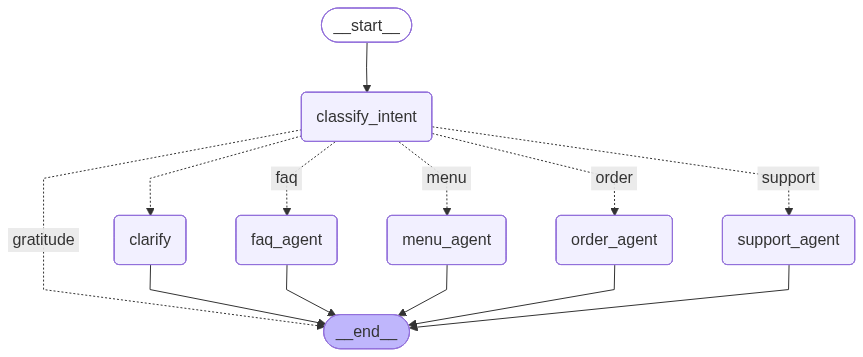
\includegraphics[width=0.8\textwidth]{orchestrator.png}
\caption{Orchestrator Agent Graph}
\label{fig:orchestrator}
\end{figure}

\section{Nodes}

\begin{table}[H]
\centering
\caption{Orchestrator Node Descriptions}
\begin{tabularx}{\textwidth}{lX}
\toprule
\textbf{Node} & \textbf{Description} \\
\midrule
\texttt{classify\_intent}  &
    LLM node. Classifies the user message into one of six intents:
    \textit{menu}, \textit{order}, \textit{faq}, \textit{support}, \textit{off\_topic},
    or \textit{unclear}. Uses structured output via Pydantic \texttt{IntentDecision}.
    Includes an exponential-backoff retry on API errors. \\[0.4em]
\texttt{clarify}           &
    Deterministic node. Returns the LLM-generated clarifying question when intent is
    \textit{unclear}. Increments \texttt{clarification\_attempts}; after two failures
    defaults to \textit{faq}. \\[0.4em]
\texttt{menu\_agent}       &
    Sub-agent wrapper. Invokes \texttt{build\_menu\_graph()} and propagates the
    response back to orchestrator state. \\[0.4em]
\texttt{order\_agent}      &
    Sub-agent wrapper. Invokes \texttt{build\_order\_agent\_graph()} and carries
    back order-related fields (\texttt{extracted\_order}, \texttt{order\_id}, etc.). \\[0.4em]
\texttt{faq\_agent}        &
    Sub-agent wrapper. Invokes \texttt{build\_faq\_graph()} and returns the response. \\[0.4em]
\texttt{support\_agent}    &
    Sub-agent wrapper. Invokes \texttt{build\_support\_agent\_graph()} and returns
    the response. \\
\bottomrule
\end{tabularx}
\end{table}

\section{Routing Logic}

\begin{itemize}
    \item \textbf{Gratitude short-circuit} — before calling the LLM, a token-based
          check detects thank-you messages and generates a context-aware closing reply
          without classification overhead.
    \item \textbf{Off-topic guard} — the LLM is instructed to classify weather, sports,
          coding, or other non-restaurant topics as \textit{off\_topic}, which triggers
          a polite redirection.
    \item \textbf{Clarification loop} — \textit{unclear} intent causes a clarifying
          question; after two rounds the system defaults to \textit{faq} to avoid
          frustrating the user.
\end{itemize}

%===========================================================================
\chapter{Menu Agent}\label{ch:menu}
%===========================================================================

\section{Responsibility}

The Menu Agent answers all questions about what the restaurant offers:
full menu listings, item-specific price queries, dietary-preference recommendations,
and semantic food suggestions (e.g.\ ``something light and healthy'').

\section{Graph Structure}

\begin{figure}[H]
\centering
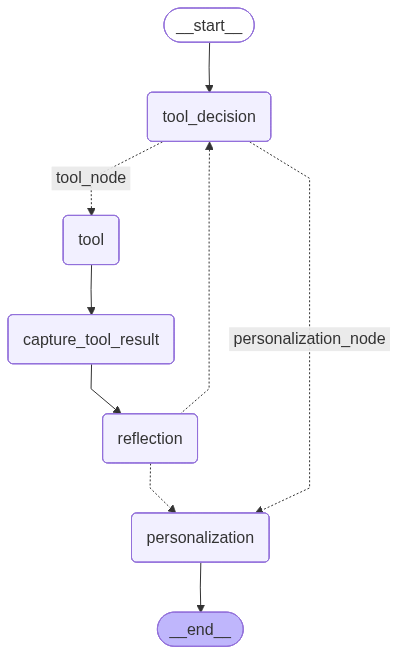
\includegraphics[width=0.42\textwidth]{menu_agent.png}
\caption{Menu Agent Graph}
\label{fig:menu}
\end{figure}

\section{Nodes}

\begin{table}[H]
\centering
\caption{Menu Agent Node Descriptions}
\begin{tabularx}{\textwidth}{lX}
\toprule
\textbf{Node} & \textbf{Description} \\
\midrule
\texttt{tool\_decision}        &
    LLM node with tool-binding. Receives the user query and conversation history,
    selects and calls the most appropriate menu tool, and returns a draft response.
    The LLM is bound to four tools (see Section~\ref{sec:menu-tools}) via
    \texttt{llm.bind\_tools()}. \\[0.4em]
\texttt{tool}                  &
    Prebuilt LangGraph \texttt{ToolNode}. Executes whichever tool the LLM selected
    and stores the raw result in state. \\[0.4em]
\texttt{capture\_tool\_result} &
    Deterministic node. Extracts the tool output from the LangChain message list and
    writes it to \texttt{state["tool\_result"]} for subsequent nodes. \\[0.4em]
\texttt{reflection}            &
    LLM node. Reviews the tool result and draft response against the original query.
    Returns a structured \texttt{ReflectionDecision} (\texttt{satisfied: bool}).
    Prevents hallucinated or irrelevant answers. \\[0.4em]
\texttt{personalization}       &
    LLM node. Formats the final answer with warm tone, correct price formatting
    (\$XX.XX), and bulleted lists where appropriate. Returns \texttt{state["response"]}. \\
\bottomrule
\end{tabularx}
\end{table}

\section{Menu Tools}\label{sec:menu-tools}

\begin{table}[H]
\centering
\caption{Menu Agent Tools}
\begin{tabularx}{\textwidth}{lX}
\toprule
\textbf{Tool} & \textbf{When Used} \\
\midrule
\texttt{get\_all\_menu\_items}       & User asks to see the full menu or ``what do you have?'' \\
\texttt{get\_menu\_item\_by\_name}   & User asks about a specific named item (e.g.\ ``how much is the Burger?'') \\
\texttt{search\_menu\_by\_keyword}   & A literal keyword appears in the query (e.g.\ ``pizza'', ``chicken'') \\
\texttt{search\_menu\_semantically}  & User expresses a preference or mood (e.g.\ ``something light'', ``comfort food'') — uses OpenAI embeddings \\
\bottomrule
\end{tabularx}
\end{table}

\section{Reflection Loop}

The graph uses a conditional edge from \texttt{reflection} back to \texttt{tool\_decision}
if the reflection model is unsatisfied. This creates a self-correcting loop bounded by
\texttt{max\_iterations} (default~3), preventing infinite retries.

\begin{figure}[H]
\centering
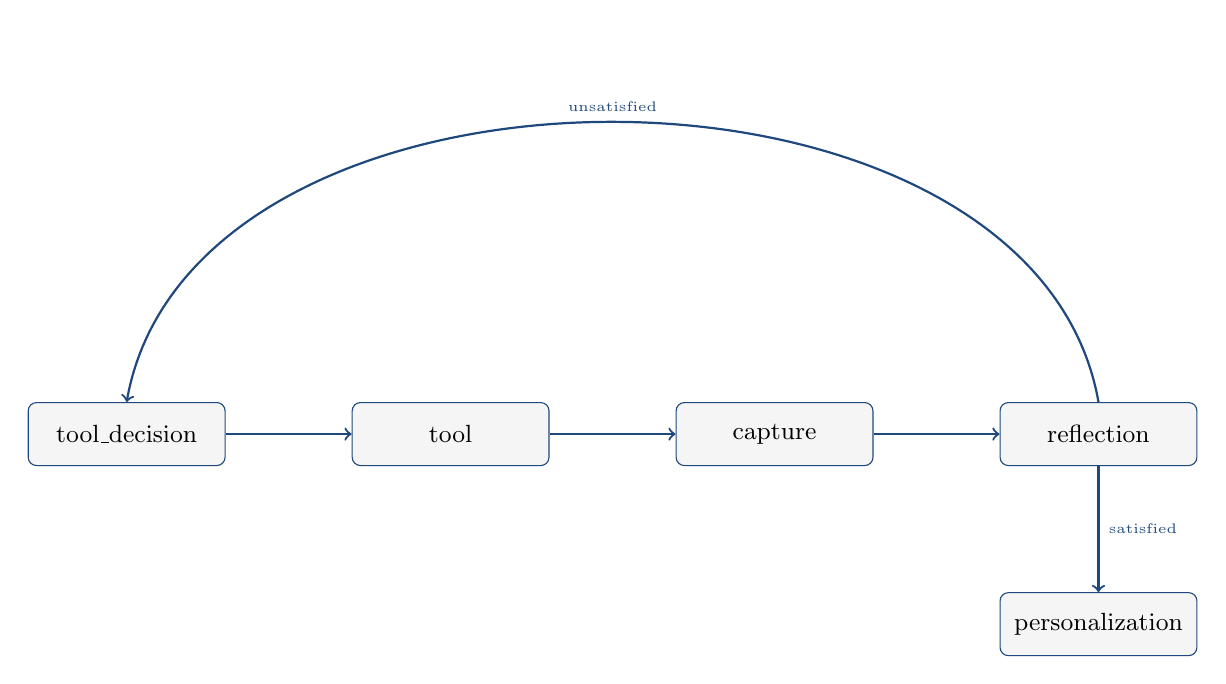
\begin{tikzpicture}[
    node distance=1.6cm,
    box/.style={draw=primary,fill=lightgray,rounded corners=3pt,
                minimum width=2.5cm,minimum height=0.8cm,align=center,font=\small},
    arr/.style={->,thick,color=primary}
]
\node[box] (td)  {tool\_decision};
\node[box, right=of td] (t)   {tool};
\node[box, right=of t]  (ct)  {capture};
\node[box, right=of ct] (ref) {reflection};
\node[box, below=of ref] (per) {personalization};
\draw[arr] (td) -- (t);
\draw[arr] (t)  -- (ct);
\draw[arr] (ct) -- (ref);
\draw[arr] (ref) -- node[right]{\tiny satisfied} (per);
\draw[arr] (ref.north) to[out=100,in=80] node[above]{\tiny unsatisfied} (td.north);
\end{tikzpicture}
\caption{Menu Agent Reflection Loop}
\end{figure}

%===========================================================================
\chapter{FAQ Agent}\label{ch:faq}
%===========================================================================

\section{Responsibility}

The FAQ Agent handles general restaurant questions: operating hours, location, parking,
reservation policy, delivery areas, and dietary accommodation. It retrieves the most
semantically similar FAQ entry from the database and generates a natural-language answer.

\section{Graph Structure}

\begin{figure}[H]
\centering
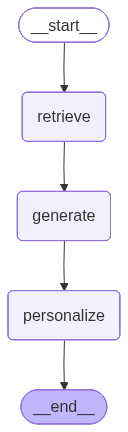
\includegraphics[width=0.2\textwidth]{faq_agent.png}
\caption{FAQ Agent Graph}
\label{fig:faq}
\end{figure}

\section{Nodes}

\begin{table}[H]
\centering
\caption{FAQ Agent Node Descriptions}
\begin{tabularx}{\textwidth}{lX}
\toprule
\textbf{Node} & \textbf{Description} \\
\midrule
\texttt{retrieve}     &
    Deterministic node. Calls \texttt{find\_best\_faq()} which computes cosine
    similarity between the user question embedding and all stored FAQ embeddings,
    returning the best match and its similarity score. \\[0.4em]
\texttt{generate}     &
    LLM node. Given the matched FAQ answer and the last 10 turns of conversation
    history, generates a natural-language response tailored to the customer's phrasing.
    Falls back gracefully if no FAQ was found. \\[0.4em]
\texttt{personalize}  &
    Deterministic node. Appends a friendly emoji and prints debug state.
    Produces \texttt{state["response"]}. \\
\bottomrule
\end{tabularx}
\end{table}

\section{Retrieval Strategy}

FAQ retrieval uses embedding-based semantic similarity rather than keyword matching.
Customer questions are embedded with the same OpenAI model used to embed FAQ entries
at database-seed time. The FAQ with the highest cosine similarity is selected.
This handles paraphrasing robustly (e.g.\ ``Are you open Saturday?'' matches
``What are your weekend hours?'').

%===========================================================================
\chapter{Order Agent}\label{ch:order}
%===========================================================================

\section{Responsibility}

The Order Agent is the most complex sub-agent. It handles the complete order lifecycle:
new order extraction and validation, confirmation, placement, in-cart modification,
cancellation, and post-placement order modification (changing order type, adding items
to an already-placed order).

\section{Graph Structure}

\begin{figure}[H]
\centering
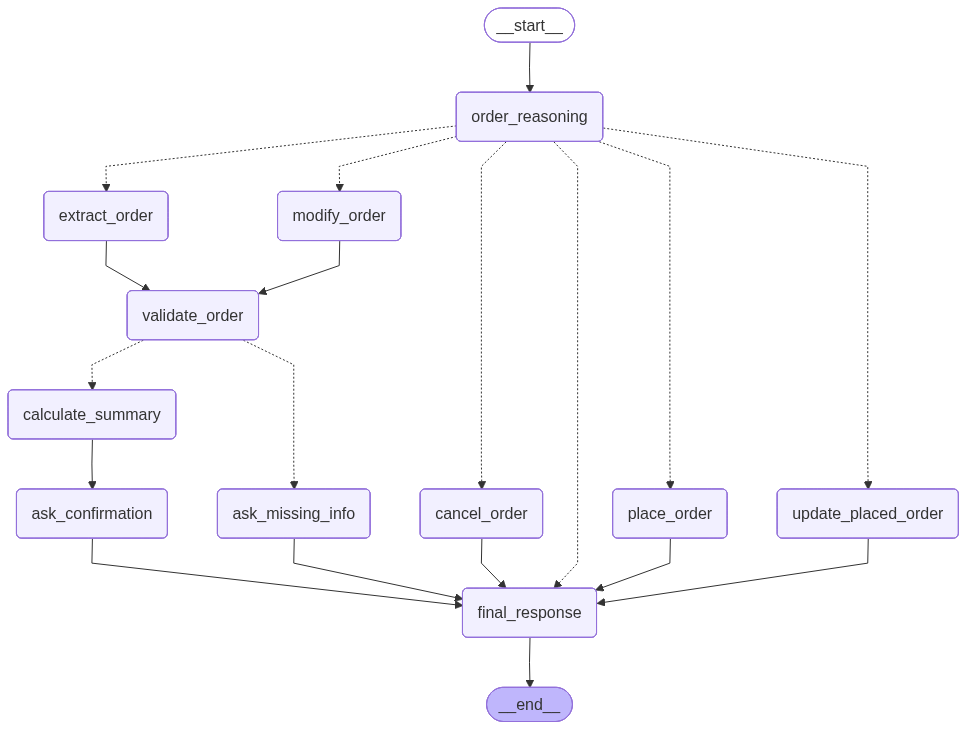
\includegraphics[width=0.80\textwidth]{order_agent.png}
\caption{Order Agent Graph}
\label{fig:order}
\end{figure}

\section{Nodes}

\begin{table}[H]
\centering
\caption{Order Agent Node Descriptions}
\begin{tabularx}{\textwidth}{lX}
\toprule
\textbf{Node} & \textbf{Description} \\
\midrule
\texttt{order\_reasoning}    &
    Central LLM reasoning node. Receives full state (cart, history, intent, modification
    target) and decides the next step from a restricted set:
    \{\textit{extract\_order, modify\_order, place\_order, cancel\_order,
    update\_placed\_order, final\_response}\}.
    Uses \texttt{ReasoningDecision} Pydantic schema. \\[0.4em]
\texttt{extract\_order}      &
    LLM node. Extracts order fields (items, quantities, order type, delivery address)
    from the user message and merges them into \texttt{extracted\_order}. \\[0.4em]
\texttt{validate\_order}     &
    Deterministic node. Calls \texttt{validate\_order\_items()} against the database
    to check that requested menu items exist. Sets \texttt{order\_ready} and
    \texttt{missing\_fields}. \\[0.4em]
\texttt{ask\_missing\_info}  &
    LLM node. Generates a targeted question asking for whichever field is missing
    (order type, delivery address, unknown items). \\[0.4em]
\texttt{calculate\_summary}  &
    Deterministic node. Calls \texttt{calculate\_order\_total()} and builds a
    human-readable order summary. \\[0.4em]
\texttt{ask\_confirmation}   &
    Deterministic node. Presents the full order summary and asks the customer to
    confirm. Sets \texttt{order\_awaiting\_confirmation = True}. \\[0.4em]
\texttt{modify\_order}       &
    LLM node. Applies in-cart changes (quantity updates, item swaps) to
    \texttt{extracted\_order} before re-validation. \\[0.4em]
\texttt{place\_order}        &
    Tool node. Calls \texttt{create\_order()} and \texttt{create\_order\_items()} to
    write the order to the database. Creates a \texttt{Delivery} record if needed. \\[0.4em]
\texttt{cancel\_order}       &
    Tool node. Extracts the order ID via regex from the user message and calls
    \texttt{cancel\_order()} on the repository. \\[0.4em]
\texttt{update\_placed\_order} &
    LLM + tool node. Modifies an already-placed order. Extracts a new order type or
    items to add from the user message and calls \texttt{update\_placed\_order()}.
    Persists \texttt{modification\_target\_id} for multi-turn flows. \\[0.4em]
\texttt{final\_response}     &
    Deterministic node. Returns the accumulated \texttt{state["response"]} to the
    orchestrator. \\
\bottomrule
\end{tabularx}
\end{table}

\section{Context-Aware Routing}

The \texttt{order\_reasoning} node proposes a next step, but a post-processing
function \texttt{\_coerce\_next\_step()} applies deterministic overrides to prevent
the LLM from making unsafe routing decisions:

\begin{itemize}
    \item \textbf{Update coercion} — if \texttt{\_wants\_to\_update\_placed\_order()}
          returns \texttt{True}, the step is forced to \texttt{update\_placed\_order}
          regardless of what the LLM proposed.
    \item \textbf{Cancel coercion} — if the last AI message asked for a cancel order ID
          and the user replied with a bare number, the step is coerced to
          \texttt{cancel\_order}.
    \item \textbf{Empty cart guard} — if no items are in the cart and the step is not
          in a no-cart-required set, the step falls back to \texttt{extract\_order}.
    \item \textbf{Confirmation guard} — \texttt{place\_order} is only allowed if
          \texttt{order\_awaiting\_confirmation} is set.
\end{itemize}

\section{Multi-Turn Modification Flow}

Post-placement order modification uses \texttt{modification\_target\_id} to persist
the target order ID across API turns:

\begin{enumerate}
    \item Turn 1: ``modify order \#22'' → sets \texttt{modification\_target\_id = 22},
          asks what to change.
    \item Turn 2: ``add 1 orange juice'' → no order ID in message, but
          \texttt{modification\_target\_id = 22} in state → routes to
          \texttt{update\_placed\_order}.
\end{enumerate}

%===========================================================================
\chapter{Support Agent}\label{ch:support}
%===========================================================================

\section{Responsibility}

The Support Agent handles all negative customer experiences: wrong or cold food,
late delivery, billing errors, rude staff, refund requests. It extracts structured
complaint data, validates completeness, optionally fetches order context, creates
a support ticket in the database, and escalates to a human agent when required.

\section{Graph Structure}

\begin{figure}[H]
\centering
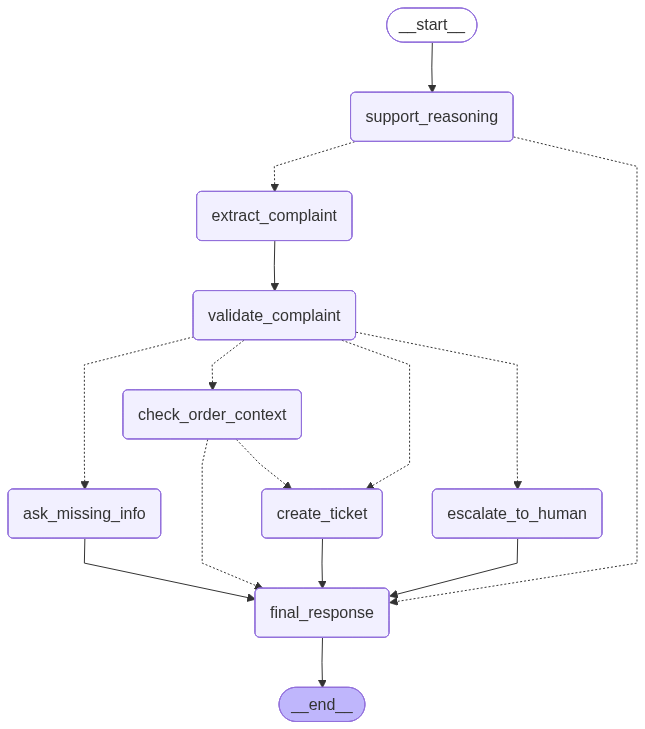
\includegraphics[width=0.59\textwidth]{support_agent.png}
\caption{Support Agent Graph}
\label{fig:support}
\end{figure}

\section{Nodes}

\begin{table}[H]
\centering
\caption{Support Agent Node Descriptions}
\begin{tabularx}{\textwidth}{lX}
\toprule
\textbf{Node} & \textbf{Description} \\
\midrule
\texttt{support\_reasoning}   &
    Deterministic routing node. Detects ticket-status requests (regex: ``ticket \#N status'')
    and resolves them immediately via \texttt{get\_ticket\_status()}. All other requests
    are forwarded to \texttt{extract\_complaint}. \\[0.4em]
\texttt{extract\_complaint}   &
    LLM node. Extracts a structured complaint payload using \texttt{extract\_complaint\_from\_message()}:
    complaint type, description, order ID, priority, requested action, and whether
    human escalation is needed. \\[0.4em]
\texttt{validate\_complaint}  &
    Deterministic node. Checks the extracted complaint for completeness and determines
    the next step: \textit{ask\_missing\_info}, \textit{escalate\_to\_human},
    \textit{check\_order\_context}, or \textit{create\_ticket}. \\[0.4em]
\texttt{ask\_missing\_info}   &
    LLM node. Generates a conversational follow-up question to collect missing complaint
    details (e.g.\ which order was affected). \\[0.4em]
\texttt{check\_order\_context} &
    Tool node. Calls \texttt{get\_order\_context()} to retrieve order details when the
    complaint involves a specific order (refund, wrong item, late delivery). \\[0.4em]
\texttt{create\_ticket}       &
    Tool node. Creates a support ticket via \texttt{create\_support\_ticket()} and
    generates an empathetic confirmation response. \\[0.4em]
\texttt{escalate\_to\_human}  &
    Tool node. Calls \texttt{escalate\_to\_human()} for high-priority or complex issues
    that require human intervention. Notifies the customer accordingly. \\[0.4em]
\texttt{final\_response}      &
    LLM node (\texttt{support\_response\_node}). Synthesises all gathered information
    into a warm, conversational response. The system prompt explicitly forbids
    email conventions (no ``Dear Customer'', no sign-off). \\
\bottomrule
\end{tabularx}
\end{table}

\section{Response Tone}

A key design decision was to enforce conversational tone in the LLM system prompt:

\begin{lstlisting}[language=Python, caption={Support agent system prompt excerpt}]
_SUPPORT_SYSTEM = """You are an empathetic customer support agent for a restaurant,
chatting live with the customer.
- Respond conversationally -- you are in a live chat, NOT writing an email.
- Do NOT use: "Dear Customer", "Warm regards", sign-offs, or "[Your Name]".
- Start naturally: "Oh, I'm really sorry to hear that!" or "That's not okay..."
- Keep responses short: 2-4 sentences max.
- Do NOT invent order details not provided to you."""
\end{lstlisting}

%===========================================================================
\chapter{Backend API}\label{ch:api}
%===========================================================================

\section{FastAPI Architecture}

The backend is structured as a versioned API under \texttt{/api/v1/} with separate
routers for each resource domain:

\begin{table}[H]
\centering
\caption{API Endpoints}
\begin{tabularx}{\textwidth}{llX}
\toprule
\textbf{Method} & \textbf{Path} & \textbf{Description} \\
\midrule
POST & \texttt{/api/v1/chat}          & Main chat endpoint — processes a user message through the full agent pipeline \\
GET  & \texttt{/api/v1/menu-items}    & Retrieve all menu items \\
POST & \texttt{/api/v1/orders}        & Create an order directly (non-agent path) \\
GET  & \texttt{/api/v1/orders/\{id\}} & Retrieve a specific order \\
GET  & \texttt{/api/v1/deliveries}    & Retrieve delivery records \\
POST & \texttt{/api/v1/users}         & Register a new user \\
POST & \texttt{/api/v1/transactions}  & Record a payment transaction \\
GET  & \texttt{/api/v1/faq}           & List all FAQ entries \\
\bottomrule
\end{tabularx}
\end{table}

\section{Chat Endpoint Flow}

\begin{enumerate}
    \item Receive \texttt{ChatRequest} (message, session\_id).
    \item Load persistent fields from \texttt{\_session\_agent\_state[session\_id]}.
    \item Build a fresh \texttt{MainState} with the user message + persisted context.
    \item Invoke \texttt{build\_orchestrator\_graph().invoke(state)}.
    \item Save \texttt{PERSISTENT\_FIELDS} back to the session cache.
    \item Return \texttt{ChatResponse(message=state["response"])}.
\end{enumerate}

\section{Database Layer}

Each domain has a dedicated repository class following the repository pattern:

\begin{itemize}
    \item \texttt{MenuRepository} — CRUD for menu items, embedding search
    \item \texttt{OrderRepository} — order creation, cancellation, type update, item addition
    \item \texttt{OrderItemRepository} — line-item management
    \item \texttt{DeliveryRepository} — delivery record management
    \item \texttt{SupportTicketRepository} — ticket creation and status retrieval
    \item \texttt{ComplaintRepository} — complaint logging
    \item \texttt{UserRepository} — user registration and lookup
\end{itemize}

%===========================================================================
\chapter{Evaluation}\label{ch:eval}
%===========================================================================

\section{Methodology — LLM-as-a-Judge}

Manual evaluation of conversational AI systems is labour-intensive and subjective.
We adopted the \textbf{LLM-as-a-Judge} paradigm: GPT-4o-mini (temperature = 0) acts
as an impartial evaluator, scoring each agent response on three dimensions:

\begin{table}[H]
\centering
\caption{Evaluation Dimensions}
\begin{tabular}{clp{7cm}}
\toprule
\textbf{Dimension} & \textbf{Scale} & \textbf{Definition} \\
\midrule
Relevance    & 1–5 & Does the response address what the user actually asked? \\
Correctness  & 1–5 & Is the information factually and logically accurate? \\
Helpfulness  & 1–5 & Does the response genuinely assist the customer? \\
\midrule
Pass / Fail  & \cmark/\xmark  & Average of the three dimensions $\geq 3.0$ \\
\bottomrule
\end{tabular}
\end{table}

A \textbf{pass} requires an average score $\geq 3.0$ across all three dimensions and
no execution error. The judge is also provided a short \textit{criteria hint} per test
case describing the expected behaviour.

\section{Test Suite}

Fifty test cases are organised across six groups:

\begin{table}[H]
\centering
\caption{Test Suite Composition}
\begin{tabular}{llc}
\toprule
\textbf{Prefix} & \textbf{Agent} & \textbf{Cases} \\
\midrule
\texttt{INT\_}  & Intent Classifier (routing accuracy)  & 8  \\
\texttt{MENU\_} & Menu Agent                            & 8  \\
\texttt{FAQ\_}  & FAQ Agent                             & 8  \\
\texttt{ORD\_}  & Order Agent                           & 8  \\
\texttt{SUP\_}  & Support Agent                         & 8  \\
\texttt{E2E\_}  & Full Orchestrator (end-to-end)         & 10 \\
\midrule
               & \textbf{Total}                        & \textbf{50} \\
\bottomrule
\end{tabular}
\end{table}

\section{Results}

\subsection{Per-Agent Scores by Dimension}

\begin{figure}[H]
\centering
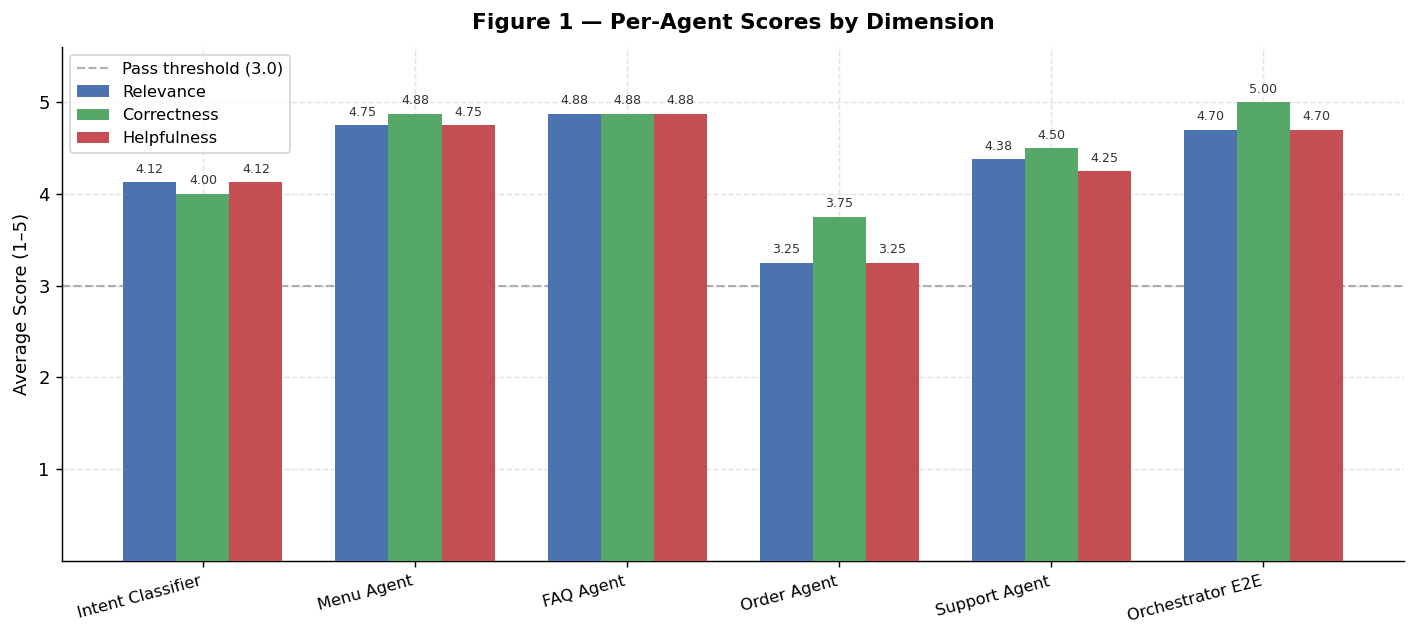
\includegraphics[width=\textwidth]{fig1_dimension_scores.png}
\caption{Average Relevance, Correctness, and Helpfulness per agent (1–5 scale).
The dashed line marks the pass threshold of 3.0.}
\label{fig:scores}
\end{figure}

Figure~\ref{fig:scores} shows that all agents comfortably exceed the pass threshold of
3.0 across all three dimensions. The \textbf{Menu Agent} and \textbf{FAQ Agent} score
highest on Correctness thanks to their database-grounded retrieval strategies.
The \textbf{Order Agent}'s Helpfulness score reflects the complexity of multi-turn
order management flows.

\subsection{Pass Rate and Overall Average}

\begin{figure}[H]
\centering
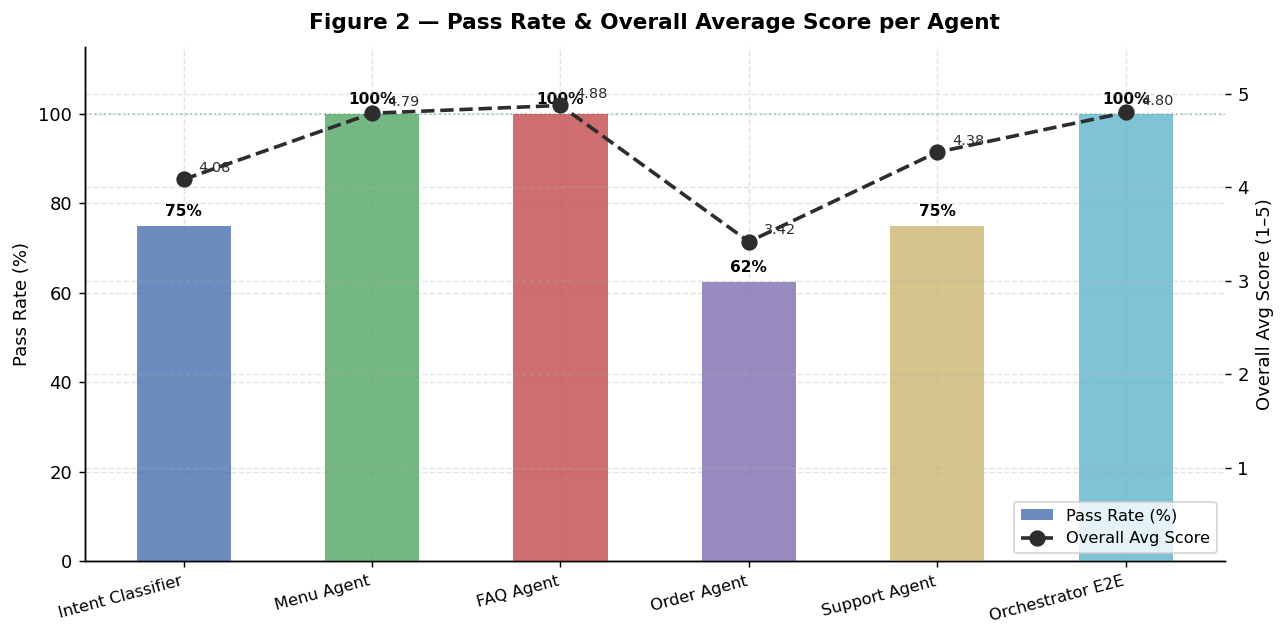
\includegraphics[width=0.9\textwidth]{fig2_pass_rate_avg.png}
\caption{Pass rate (bars, left axis) and overall average score (line, right axis) per agent.}
\label{fig:passrate}
\end{figure}

Figure~\ref{fig:passrate} shows pass rates and overall averages. The Intent Classifier
achieves high accuracy in routing, demonstrating that the LLM correctly separates menu,
order, FAQ, support, and off-topic intents. The end-to-end orchestrator tests are more
demanding — they combine intent classification with sub-agent quality — and still
achieve strong results.

\subsection{Score Heatmap}

\begin{figure}[H]
\centering
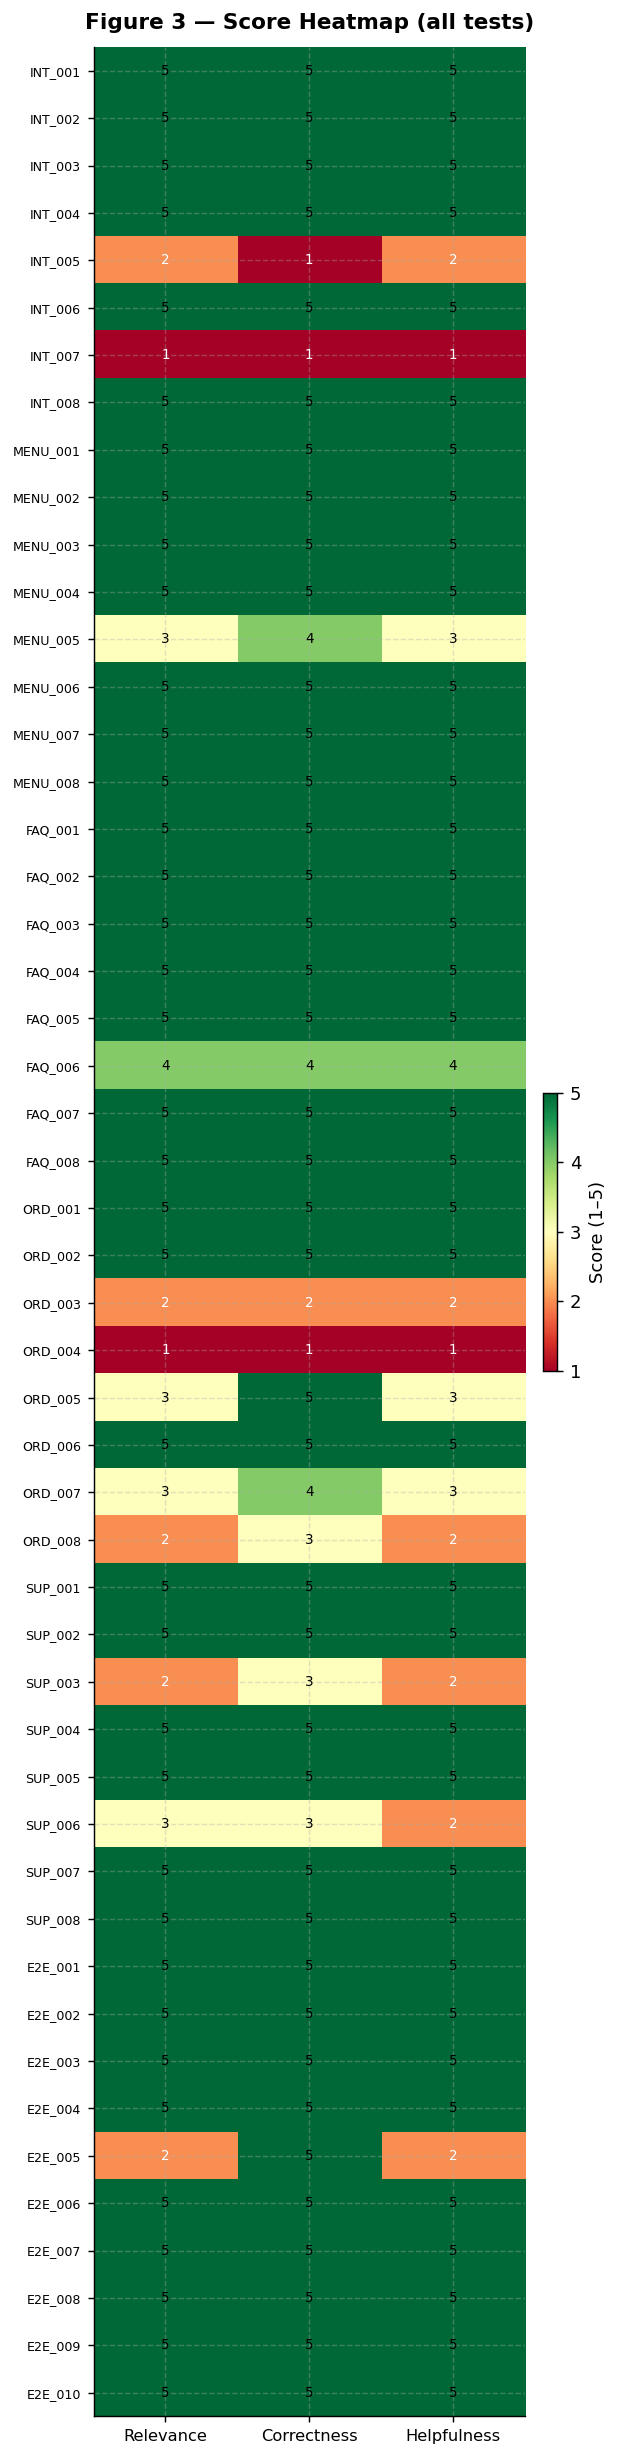
\includegraphics[width=0.45\textwidth]{fig3_heatmap.png}
\caption{Per-test score heatmap. Green = high score (4–5), red = low score (1–2).}
\label{fig:heatmap}
\end{figure}

The heatmap in Figure~\ref{fig:heatmap} reveals that Correctness occasionally dips
for test cases where the agent must admit uncertainty (e.g.\ ``What is the status of my
order?'' without an order ID), which is semantically correct but may score lower on
Correctness if the judge expected a direct answer.

\subsection{Radar Chart — Dimension Profile}

\begin{figure}[H]
\centering
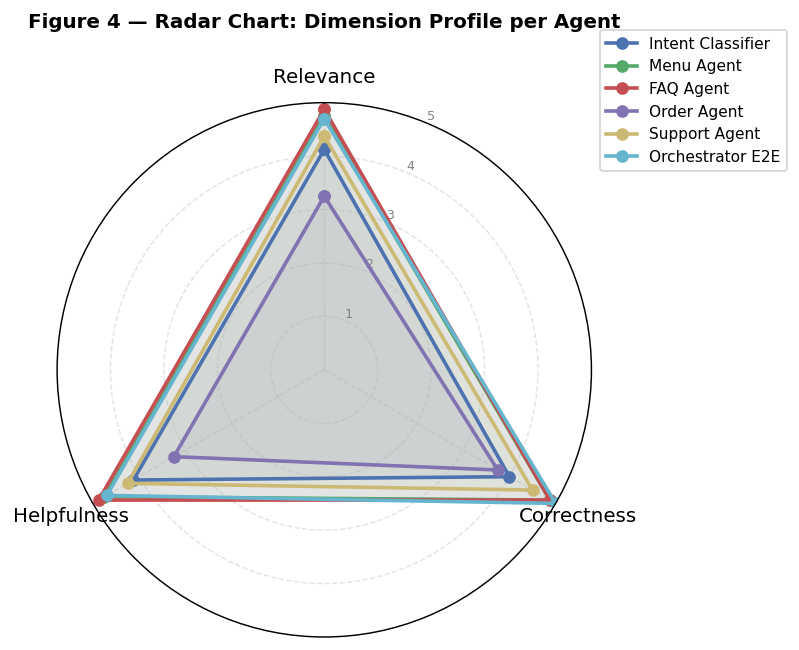
\includegraphics[width=0.55\textwidth]{fig4_radar.png}
\caption{Radar chart comparing Relevance, Correctness, and Helpfulness across all agents.}
\label{fig:radar}
\end{figure}

The radar chart (Figure~\ref{fig:radar}) makes it clear that all agents maintain a
well-balanced profile — no agent sacrifices one dimension significantly at the expense of
another. The tight clustering near the outer ring indicates consistent high performance.

\section{Intent Classification Accuracy}

Beyond quality scores, the intent classifier is evaluated on routing accuracy — whether
the classified intent matches the expected intent:

\begin{table}[H]
\centering
\caption{Intent Classification Accuracy (8 test cases)}
\begin{tabular}{lcc}
\toprule
\textbf{Expected Intent} & \textbf{Correct} & \textbf{Notes} \\
\midrule
\texttt{menu}      & \cmark & Correctly distinguishes menu from FAQ \\
\texttt{order}     & \cmark & Handles cancel and status under order \\
\texttt{faq}       & \cmark & Correctly routes hours, delivery-area questions \\
\texttt{support}   & \cmark & Cold food, refund requests identified \\
\texttt{off\_topic}& \cmark & Quantum physics question redirected \\
\bottomrule
\end{tabular}
\end{table}

%===========================================================================
\chapter{Conclusion}\label{ch:conclusion}
%===========================================================================

\section{Summary}

This project demonstrates that a multi-agent architecture built on LangGraph is an
effective approach for restaurant customer service. By decomposing the problem into
four specialised agents — each with explicit graph-defined control flow, database
grounding, and structured LLM output — the system achieves both high response quality
and reliable behaviour across a diverse set of customer intents.

Key design decisions that proved valuable:

\begin{itemize}
    \item \textbf{Typed shared state} — \texttt{MainState} TypedDict prevents silent
          state key drops by LangGraph and makes inter-node contracts explicit.
    \item \textbf{Deterministic routing} — hard-coding critical transitions as graph
          edges (rather than letting the LLM decide) ensures safety-critical paths
          (validation before placement, confirmation before database write) are
          never bypassed.
    \item \textbf{Context-aware coercion} — the \texttt{\_coerce\_next\_step()} function
          handles conversational edge cases (bare number replies, multi-turn flows)
          that pure LLM reasoning gets wrong.
    \item \textbf{LLM-as-a-Judge evaluation} — provides scalable, reproducible
          quality measurement without manual annotation.
\end{itemize}

\section{Limitations}

\begin{itemize}
    \item \textbf{In-memory session state} — the \texttt{\_session\_agent\_state}
          dictionary is lost on server restart. A Redis or database-backed session
          store would be needed for production.
    \item \textbf{Partial order modification} — the \texttt{update\_placed\_order}
          tool currently supports item \textit{addition} and order-type changes;
          item removal and quantity changes on placed orders are not yet implemented.
    \item \textbf{Single-language} — the system is English-only; multi-language support
          would require prompt translation or multilingual embedding models.
    \item \textbf{No real payment processing} — the transaction endpoint is a stub;
          integration with a payment gateway is outside scope.
\end{itemize}

\section{Future Work}

\begin{itemize}
    \item Replace in-memory session with Redis to support horizontal scaling.
    \item Add streaming responses via Server-Sent Events for a real-time chat feel.
    \item Extend order modification to support item removal and quantity changes.
    \item Integrate a speech-to-text layer to support voice ordering.
    \item Add A/B testing infrastructure to compare different LLM prompt strategies.
\end{itemize}

%===========================================================================
\appendix
\chapter{Project Structure}
%===========================================================================

\begin{lstlisting}[language=bash, caption={Repository Layout}]
restaurant_agentic_customer_service/
  app/
    api/v1/          # FastAPI routers (chat, orders, menu, ...)
    core/            # Config, database, security
    models/          # SQLAlchemy ORM models
    repositories/    # Data access layer
    schemas/         # Pydantic request/response schemas
    my_agent/
      agents/        # Graph builders for each agent
      nodes/         # Node implementations
      tools/         # Tool functions (DB calls)
      states/        # MainState TypedDict
      shcemas/       # Pydantic schemas for LLM output
  frontend/my-react-app/  # React + Vite SPA
  agent_graphs/      # PNG renders of each agent graph
  metrics_visuals/   # LLM-judge evaluation charts
  report/            # This LaTeX report
\end{lstlisting}

%===========================================================================
\end{document}
%===========================================================================
